\documentclass[10pt,a4paper]{article}
\usepackage[margin=2.2cm]{geometry}
\usepackage{amsmath,amssymb}
\usepackage{lmodern}
\usepackage[T1]{fontenc}
\usepackage{booktabs,array}
\usepackage{graphicx}
\usepackage{tikz}
\usetikzlibrary{decorations.pathreplacing,arrows.meta,calc}
\usepackage[font=small,labelfont=bf]{caption}
\usepackage[colorlinks=true,linkcolor=blue!50!black,urlcolor=blue!50!black]{hyperref}

\definecolor{regc}{RGB}{31,119,180}
\definecolor{tailc}{RGB}{214,39,40}
\newcommand{\code}[1]{\texttt{\small #1}}
\newcommand{\Qp}{Q'}

\title{The final mesh interval of the sampled-data solvers in \texttt{voles}}
\author{Implementation note (voles 1.0)}
\date{14 November 2026}

\renewcommand{\topfraction}{0.9}\renewcommand{\bottomfraction}{0.8}
\renewcommand{\textfraction}{0.08}\renewcommand{\floatpagefraction}{0.8}

\begin{document}
\maketitle

\noindent
The array-input solvers (\code{solve\_vie1/2/vide} with sampled \code{kernel}, \code{g}, \code{a})
use a uniform mesh of $Q$ samples per interval. The record need not end on a mesh point:
when $N-1$ is not a multiple of $Q$, the last regular interval and the $r$ leftover samples
are merged into one longer \emph{final interval}, with its own collocation nodes snapped to the
sample grid and its own collocation row, solved after the regular intervals. No data are discarded.
This note describes that construction as implemented in
\code{\_product.mesh\_split}, \code{\_product.snap\_nodes}, \code{\_product.solve\_tail},
\code{\_sampled.\_with\_tail} and \code{\_product.\_finish}.

\section{Notation}

\begin{center}
\small
\renewcommand{\arraystretch}{1.18}
\begin{tabular}{>{$}l<{$} p{9.9cm} l}
\toprule
\text{Symbol} & Meaning & Code \\
\midrule
\delta & sample spacing & \code{dt}, \code{delta} \\
N & number of samples; $t_j = j\delta$, $j = 0,\dots,N-1$; $T = (N-1)\delta$ & \code{N} \\
K_j,\ g_j,\ a_j & data samples $K(t_j)$, $g(t_j)$, $a(t_j)$ (scalars or $d\times d$ / $d$ blocks) & \code{kernel}, \code{g}, \code{a} \\
q & number of divisions of the reference interval & \code{divs} \\
k_1<\dots<k_m & the chosen node indices, $k_i\in\{0,\dots,q\}$; $m$ nodes & \code{choices} \\
c_i = k_i/q & nominal collocation nodes in $[0,1]$ & \code{nodes} \\
Q & samples per regular interval (a multiple of $q$) & \code{samples\_per\_interval} \\
H = Q\delta & width of a regular interval & \\
M_{\rm reg},\ r & $N-1 = M_{\rm reg}Q + r$, \ $0\le r<Q$ & \\
M & number of regular intervals: $M_{\rm reg}$ if $r=0$, else $M_{\rm reg}-1$ & \code{M} \\
t_l = lH & mesh points; regular intervals $I_l = [t_l, t_{l+1}]$, $l = 0,\dots,M-1$ & \\
\Qp = Q + r & samples in the final interval ($Q < \Qp < 2Q$) & \code{Qp} \\
h = \Qp\delta & width of the final interval $I_M = [t_M, T]$, \ $H < h < 2H$ & \\
\kappa_i & sample offset of the $i$-th node in $I_M$ (the snapped node) & \code{kap} \\
c'_i = \kappa_i/\Qp & snapped local nodes; collocation points $\tau_i = t_M + \kappa_i\delta$ & \code{node\_times[-1]} \\
v & local variable on $I_M$: $s = t_M + v h$, $v\in[0,1]$ & \\
L_k(v) & Lagrange basis on $\{c'_1,\dots,c'_m\}$ (on $\{0,c'_1,\dots,c'_m\}$ for the continuous VIE-1) & \code{basis\_p} \\
u_l & collocation solution on $I_l$ (local monomial coefficients) & \code{unit\_reg}, \code{unit\_t} \\
U_k & unknowns of the final row: $U_k = u_M(\tau_k)$ & \code{U} \\
p & kernel interpolation degree: \code{kernel\_interp\_degree} (product), $m$ (collocation) & \code{p} \\
K_h & piecewise degree-$p$ interpolant of the samples $K_j$ (below) & \code{coef} \\
\eta_i & history term at $\tau_i$ (contribution of $I_0,\dots,I_{M-1}$) & \code{hist} \\
A_{ik} & local block: weight of $U_k$ in the integral over $[t_M,\tau_i]$ & \code{Ab} \\
y_{\rm prev} & $u_{M-1}(t_M^-)$, or $y_0$ if $M = 0$ (continuous VIE-1, VIDE) & \code{y\_prev} \\
\bottomrule
\end{tabular}
\end{center}

\section{Splitting the record}

\code{mesh\_split(N, Q)} returns $(M, \Qp)$ from
\[
  N - 1 = M_{\rm reg}\,Q + r ,\qquad
  (M,\Qp) = \begin{cases} (M_{\rm reg},\,0) & r = 0 \quad\text{(no final interval)},\\
                          (M_{\rm reg}-1,\,Q+r) & r > 0. \end{cases}
\]
The final interval is therefore the last \emph{full} interval stretched over the leftover samples,
not a short interval of $r$ samples: its width stays within $(H, 2H)$. (A short interval of
$r \ll Q$ samples would make the first-kind local system nearly singular, since $A = O(h)$.) If $M_{\rm reg} = 1$ and $r>0$ the whole record is a single stretched interval ($M=0$).
The only constraint is $N \ge Q+1$. The regular intervals are solved exactly as before
(D or Numba driver for \code{quadrature="collocation"}, the lag-block driver for \code{"product"});
the final row is assembled and solved afterwards in NumPy.

\begin{figure}[h]
\centering
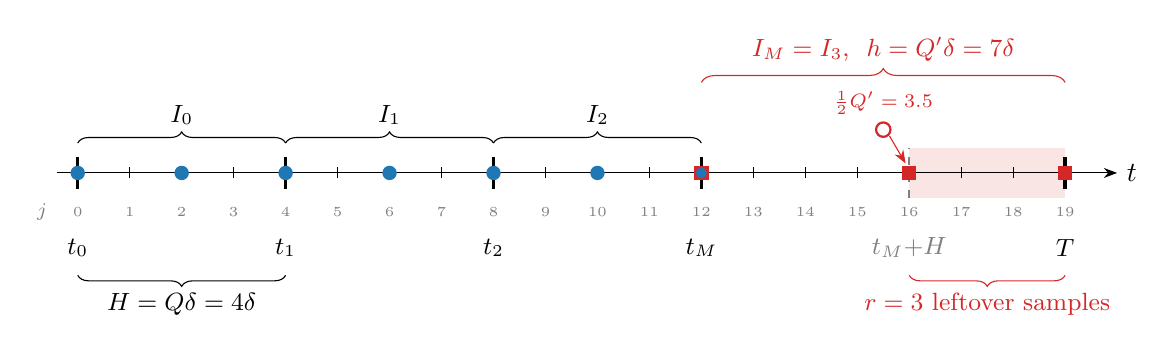
\begin{tikzpicture}[x=0.66cm,y=1cm,>=Stealth]
  % leftover samples
  \fill[tailc!12] (16,-0.32) rectangle (19,0.32);
  \draw[->] (-0.4,0) -- (20.0,0) node[right] {$t$};
  \foreach \j in {0,...,19} {
    \draw (\j,-0.07) -- (\j,0.07);
    \node[font=\tiny,gray] at (\j,-0.5) {\j};
  }
  \node[font=\scriptsize,gray,anchor=east] at (-0.4,-0.5) {$j$};
  % mesh points
  \foreach \x in {0,4,8,12} \draw[very thick] (\x,-0.2) -- (\x,0.2);
  \draw[very thick] (19,-0.2) -- (19,0.2);
  \draw[thick,dashed,gray] (16,-0.32) -- (16,0.32);
  % regular nodes (offsets 0,2,4 of each interval)
  \foreach \x in {0,2,4,6,8,10,12} \fill[regc] (\x,0) circle (2.6pt);
  % tail nodes
  \foreach \x in {12,16,19} \fill[tailc] ($(\x,0)+(-2.6pt,-2.6pt)$) rectangle ($(\x,0)+(2.6pt,2.6pt)$);
  \fill[regc] (12,0) circle (2.0pt);
  % nominal midpoint of the stretched interval
  \draw[tailc,thick] (15.5,0.55) circle (2.6pt);
  \draw[->,tailc] (15.62,0.47) -- (15.93,0.12);
  \node[tailc,font=\scriptsize,anchor=south] at (15.5,0.62) {$\tfrac12\Qp = 3.5$};
  % braces
  \foreach \a/\b/\l in {0/4/0,4/8/1,8/12/2}
    \draw[decorate,decoration={brace,amplitude=4pt}] (\a,0.38) -- (\b,0.38)
      node[midway,above=3pt,font=\small] {$I_{\l}$};
  \draw[decorate,decoration={brace,amplitude=5pt},tailc] (12,1.15) -- (19,1.15)
      node[midway,above=4pt,font=\small] {$I_M = I_3$, \ $h = \Qp\delta = 7\delta$};
  \foreach \x/\l in {0/t_0,4/t_1,8/t_2,12/t_M,19/T} \node[font=\small] at (\x,-0.95) {$\l$};
  \node[font=\small,gray] at (16,-0.95) {$t_M{+}H$};
  \draw[decorate,decoration={brace,amplitude=4pt,mirror}] (0,-1.3) -- (4,-1.3)
      node[midway,below=3pt,font=\small] {$H = Q\delta = 4\delta$};
  \draw[decorate,decoration={brace,amplitude=4pt,mirror},tailc] (16,-1.3) -- (19,-1.3)
      node[midway,below=3pt,font=\small] {$r = 3$ leftover samples};
\end{tikzpicture}
\caption{Splitting for $(q,\{k_i\}) = (2,\{0,1,2\})$ with \code{quadrature="collocation"}
($Q = q^2 = 4$) and $N = 20$: $19 = 4\cdot4 + 3$, so $M = 3$ regular intervals and a final
interval of $\Qp = 7$ samples. Blue circles: collocation points of the regular intervals
(sample offsets $k_iQ/q = 0,2,4$). Red squares: snapped nodes of the final interval,
$\kappa = (0,4,7)$; the nominal midpoint $3.5$ (hollow) is a tie and rounds up to $4$.
The dashed line is where the last regular mesh point would have been.}
\end{figure}

\section{Snapping the nodes}

On $I_M$ the nominal node $c_i$ would lie $k_i\Qp/q$ samples from $t_M$, generally not a sample.
\code{snap\_nodes} moves it to the nearest sample, ties rounding up:
\[
  \kappa_i = \Big\lfloor \frac{k_i\,\Qp}{q} + \frac12 \Big\rfloor,\qquad
  c'_i = \frac{\kappa_i}{\Qp},\qquad
  \tau_i = t_M + \kappa_i\,\delta .
\]
Properties:
\begin{itemize}\setlength\itemsep{1pt}
\item $k_i = 0 \mapsto \kappa_i = 0$ and $k_i = q \mapsto \kappa_i = \Qp$: the end nodes stay at the interval ends.
\item $|c'_i - c_i| \le 1/(2\Qp)$, i.e.\ each collocation point moves by at most $\delta/2$.
\item The $\kappa_i$ are distinct: since $\Qp > Q \ge q$, consecutive scaled nodes differ by more than one sample and rounding is monotone.
\item Exact in floating point: a tie is an integer plus $\tfrac12$ (exactly representable); a non-tie is at least $1/(2q)$ from a half-integer.
\item Ties occur only for even $q$, when $k_i\Qp/q$ has denominator $2$. All ties move right, so a node set symmetric under $c\mapsto 1-c$ generally loses that symmetry.
\item $g$ and $a$ are only needed at samples ($g_i = g_{MQ+\kappa_i}$), so they are never interpolated; $K$ enters the local blocks through its interpolant $K_h$.
\end{itemize}

\begin{figure}[h]
\centering
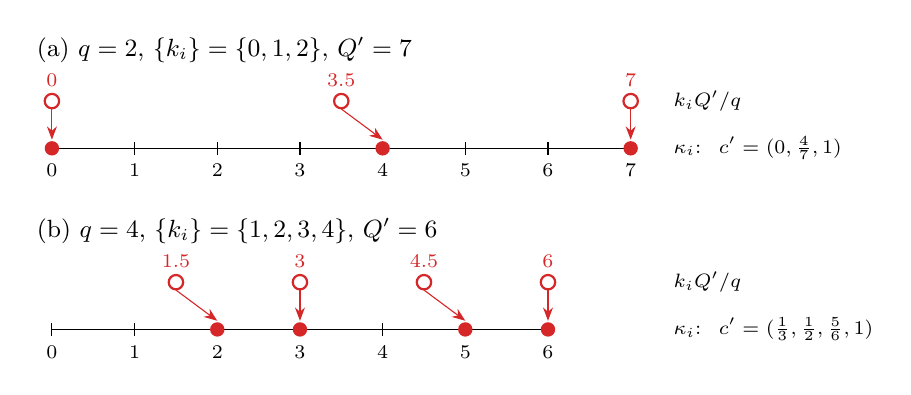
\begin{tikzpicture}[x=1.05cm,y=1cm,>=Stealth]
  \begin{scope}
    \node[anchor=west,font=\small] at (-0.3,1.25) {(a) $q=2$, $\{k_i\}=\{0,1,2\}$, $\Qp = 7$};
    \draw (0,0) -- (7,0);
    \foreach \j in {0,...,7} {\draw (\j,-0.08)--(\j,0.08); \node[font=\scriptsize,below] at (\j,-0.08) {\j};}
    \foreach \x/\lab in {0/0, 3.5/3.5, 7/7} {
      \draw[tailc,thick] (\x,0.6) circle (2.6pt);
      \node[font=\scriptsize,tailc,above] at (\x,0.66) {\lab};}
    \foreach \x/\y in {0/0, 3.5/4, 7/7} \draw[->,tailc] (\x,0.5) -- (\y,0.11);
    \foreach \x in {0,4,7} \fill[tailc] (\x,0) circle (2.6pt);
    \node[font=\scriptsize,anchor=west] at (7.4,0.6) {$k_i\Qp/q$};
    \node[font=\scriptsize,anchor=west] at (7.4,0.0) {$\kappa_i$: \ $c' = (0,\tfrac47,1)$};
  \end{scope}
  \begin{scope}[yshift=-2.3cm]
    \node[anchor=west,font=\small] at (-0.3,1.25) {(b) $q=4$, $\{k_i\}=\{1,2,3,4\}$, $\Qp = 6$};
    \draw (0,0) -- (6,0);
    \foreach \j in {0,...,6} {\draw (\j,-0.08)--(\j,0.08); \node[font=\scriptsize,below] at (\j,-0.08) {\j};}
    \foreach \x/\lab in {1.5/1.5, 3/3, 4.5/4.5, 6/6} {
      \draw[tailc,thick] (\x,0.6) circle (2.6pt);
      \node[font=\scriptsize,tailc,above] at (\x,0.66) {\lab};}
    \foreach \x/\y in {1.5/2, 3/3, 4.5/5, 6/6} \draw[->,tailc] (\x,0.5) -- (\y,0.11);
    \foreach \x in {2,3,5,6} \fill[tailc] (\x,0) circle (2.6pt);
    \node[font=\scriptsize,anchor=west] at (7.4,0.6) {$k_i\Qp/q$};
    \node[font=\scriptsize,anchor=west] at (7.4,0.0) {$\kappa_i$: \ $c' = (\tfrac13,\tfrac12,\tfrac56,1)$};
  \end{scope}
\end{tikzpicture}
\caption{Snapping on the final interval. Hollow: nominal positions $k_i\Qp/q$ in samples;
filled: $\kappa_i$. In (b) both ties ($1.5$, $4.5$) move right; the nominal pair
$\{\tfrac14,\tfrac34\}$, symmetric about $\tfrac12$, becomes $\{\tfrac13,\tfrac56\}$.}
\end{figure}

\begin{center}
\small
\begin{tabular}{lcl}
\toprule
Setting & $Q$ & snapped $c'$ by $r$ \\
\midrule
$(2,\{0,1,2\})$, product (VIE-2/VIDE default) & 2 & $r=1$: $(0,\tfrac23,1)$ \ (tie) \\
$(2,\{0,1,2\})$, collocation & 4 & $r=1$: $(0,\tfrac35,1)$; \ $r=2$: $(0,\tfrac12,1)$; \ $r=3$: $(0,\tfrac47,1)$ \\
$(3,\{1,2,3\})$, product (VIE-1 default) & 9 & no ties; e.g.\ $r=1$: $(\tfrac3{10},\tfrac7{10},1)$, \ $r=3$: $(\tfrac13,\tfrac23,1)$ \\
\bottomrule
\end{tabular}
\end{center}

\section{The collocation row of the final interval}

We write the VIE-2, $y(t) = g(t) + \int_0^t K(t-s)\,y(s)\,ds$; the other kinds follow at the end.
On $I_M$ the approximation is $u_M(t_M + vh) = \sum_{k=1}^m U_k L_k(v)$, and the collocation
equations at $\tau_1,\dots,\tau_m$ split the integral at $t_M$:
\[
  U_i \;=\; g(\tau_i) \;+\; \underbrace{\sum_{l=0}^{M-1}\int_{I_l} K(\tau_i - s)\,u_l(s)\,ds}_{\eta_i\ \text{(history)}}
        \;+\; \underbrace{\sum_{k=1}^m U_k \int_{t_M}^{\tau_i} K_h(\tau_i - s)\,L_k\!\Big(\frac{s-t_M}{h}\Big)ds}_{\sum_k A_{ik}U_k\ \text{(local)}} ,
  \qquad i = 1,\dots,m,
\]
i.e.\ the $m\times m$ (or $md\times md$) system $(I - A)\,U = g(\tau) + \eta$. The $u_l$, $l<M$, are known.

\begin{figure}[h]
\centering
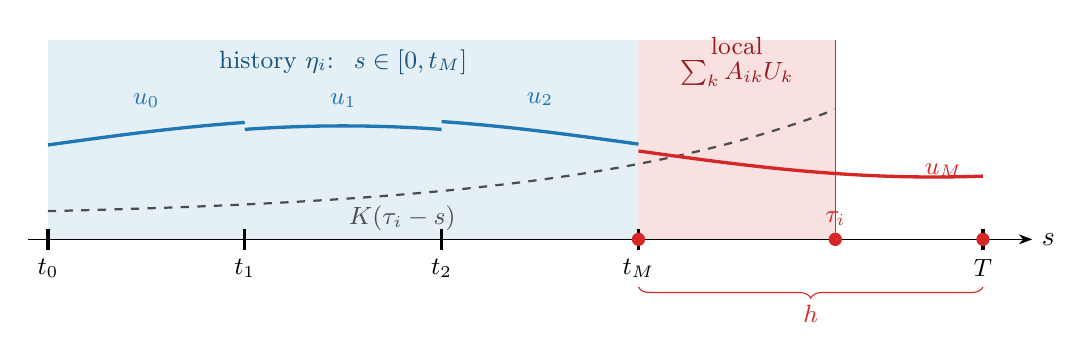
\begin{tikzpicture}[x=1.25cm,y=1.1cm,>=Stealth]
  \fill[regc!12] (0,0) rectangle (6,2.3);
  \fill[tailc!14] (6,0) rectangle (8,2.3);
  \node[regc!70!black,font=\small] at (3,2.05) {history $\eta_i$: \ $s\in[0,t_M]$};
  \node[tailc!70!black,font=\small,align=center] at (7,2.05) {local\\[-2pt] $\sum_k A_{ik}U_k$};
  \draw[->] (-0.2,0) -- (10.0,0) node[right] {$s$};
  \foreach \x/\l in {0/t_0,2/t_1,4/t_2,6/t_M} {\draw[very thick] (\x,-0.12) -- (\x,0.12); \node[below,font=\small] at (\x,-0.12) {$\l$};}
  \draw[very thick] (9.5,-0.12) -- (9.5,0.12); \node[below,font=\small] at (9.5,-0.12) {$T$};
  % kernel K(tau_i - s), tau_i = 8
  \draw[thick,dashed,black!70,domain=0:8,samples=60] plot (\x,{0.25+1.25*exp(-0.35*(8-\x))});
  \node[font=\small,black!70] at (3.6,0.24) {$K(\tau_i - s)$};
  % solution pieces with small jumps at the mesh points
  \foreach \a/\b/\o in {0/2/0.04,2/4/-0.04,4/6/0.05}
    \draw[regc,very thick,domain=\a:\b,samples=30] plot (\x,{1.05+0.3*sin(30*\x)+\o});
  \draw[tailc,very thick,domain=6:9.5,samples=40] plot (\x,{1.05+0.3*sin(30*\x)-0.03});
  \node[regc,font=\small] at (1.0,1.6) {$u_0$};
  \node[regc,font=\small] at (3.0,1.6) {$u_1$};
  \node[regc,font=\small] at (5.0,1.62) {$u_2$};
  \node[tailc,font=\small] at (9.1,0.8) {$u_M$};
  % collocation points of I_M: kappa = (0,4,7) on 3.5 units => delta = 0.5
  \foreach \x/\l in {6/\tau_1,8/\tau_2,9.5/\tau_3} \fill[tailc] (\x,0) circle (2.4pt);
  \node[tailc,above,font=\small] at (8,0.05) {$\tau_i$};
  \draw[tailc,thin] (8,0) -- (8,2.3);
  \draw[decorate,decoration={brace,amplitude=4pt,mirror},tailc] (6,-0.55) -- (9.5,-0.55)
      node[midway,below=3pt,font=\small] {$h$};
\end{tikzpicture}
\caption{The two parts of the integral at a collocation point $\tau_i$ of the final interval
(schematic, $M=3$). Over the regular intervals (blue) the known pieces $u_l$, which may jump at
the mesh points, are integrated against the kernel to give $\eta_i$; over $[t_M,\tau_i]$ (red)
the unknown $u_M$ enters through the local blocks $A_{ik}$.}
\end{figure}

\paragraph{Kernel interpolant.} On each cell $[t_j,t_{j+1}]$, $K_h$ is the degree-$p$ polynomial
through the $p+1$ samples nearest the cell (one-sided at the ends of the array)
(\code{interp\_cell\_coefs}). With $\Lambda_{k,c,\rho} = \int_{\text{cell }c} L_k(v)\,\xi^\rho$
the moment tensor of the snapped basis on the $\Qp$ cells of $I_M$ ($\xi\in[0,1]$ the cell variable),
the local blocks are exact integrals of piecewise polynomials:
\[
  A_{ik} = \delta \sum_{c=0}^{\kappa_i-1}\ \sum_{\rho=0}^{p}\ K_{h,\rho}^{(\kappa_i-1-c)}\,\Lambda_{k,c,\rho},
  \qquad A_{ik} = 0 \ \text{ if } \kappa_i = 0 ,
\]
where $K_{h,\rho}^{(j)}$ is the $\rho$-th monomial coefficient of $K_h$ on cell $j$ (\code{\_tail\_local\_blocks}).
The local blocks use product integration on \emph{both} quadrature paths.

\paragraph{History term.} This is where the two quadratures differ.
\begin{itemize}\setlength\itemsep{2pt}
\item \code{quadrature="product"}: $\eta_i = \sum_{l<M}\int_{I_l} K_h(\tau_i-s)\,u_l(s)\,ds$, integrated exactly,
with $K_h$ the interpolant of the \emph{full} sample array (\code{\_tail\_history}).
\item \code{quadrature="collocation"}: the interpolatory rule the regular rows use,
\[
  \eta_i = H\sum_{l=0}^{M-1}\sum_{k} b_k\,K(\tau_i - t_l - \hat c_k H)\,u_l(t_l + \hat c_k H),
  \qquad b_k = \int_0^1 \ell_k(v)\,dv ,
\]
with $\ell_k$ the Lagrange basis on the regular nodes $\hat c = (c_1,\dots,c_m)$
(prefixed by $0$ for the continuous VIE-1) (\code{\_tail\_history\_node\_rule}).
Every kernel argument $\big((M-l)Q + \kappa_i - \hat k Q/q\big)\delta$ is a sample.
Using the same rule as the regular rows matters for the first kind: a quadrature mismatch
between rows is amplified by $\sim\!1/H$ and was measured to cost one order.
\end{itemize}

\paragraph{The other equation kinds.} With $g_i = g(\tau_i)$:
\begin{itemize}\setlength\itemsep{2pt}
\item VIE-1 (discontinuous): \ $A\,U = g - \eta$.
\item VIE-1 (continuous): basis $L_0,\dots,L_m$ on $\{0,c'_1,\dots,c'_m\}$ with $U_0 = y_{\rm prev}$ fixed:
  $\sum_{k\ge1}A_{ik}U_k = g_i - \eta_i - A_{i0}\,y_{\rm prev}$.
\item VIDE, $y' = a\,y + g + \int_0^t K(t-s)\,y(s)\,ds$: \
  $u_M(t_M+vh) = y_{\rm prev} + h\sum_k Y_k\,\beta_k(v)$, $\beta_k(v) = \int_0^v L_k$, $Y_k = u_M'(\tau_k)$, and
  \[
    Y_i - \sum_k\big[A_{ik} + h\,a(\tau_i)\,\beta_k(c'_i)\big]Y_k = g_i + \eta_i + \big(A_{i0} + a(\tau_i)\big)\,y_{\rm prev},
  \]
  where here $A_{ik}$ integrates $K_h$ against $h\beta_k$ and $A_{i0} = \int_{t_M}^{\tau_i}K_h(\tau_i-s)\,ds$.
\end{itemize}
For systems ($d>0$) every entry is a $d\times d$ block, and the system is $md\times md$.

\section{Assembling the output}

\begin{itemize}\setlength\itemsep{2pt}
\item Samples $j \le MQ-1$: from the regular intervals. Samples $j = MQ+1,\dots,N-1$: $y_j = u_M(t_j)$.
\item The shared mesh point $j = MQ$: $y_{MQ} = \tfrac12\big(u_{M-1}(t_M^-) + u_M(t_M^+)\big)$
  (the same convention as at every interior breakpoint of a discontinuous solution).
\item The \code{VolterraSolution} has $M+1$ pieces with \code{mesh} $= (0, H, \dots, MH, T)$;
  \code{node\_times[-1]} holds the snapped $\tau_i$, while \code{nodes} keeps the nominal $c_i$.
\item With \code{quadrature="collocation"} the regular part is computed from \code{kernel[:MQ+1]}
  and is bit-identical to a solve on the truncated record. With \code{"product"}, $K_h$ is built
  from the full array, so cells near $t_M$ get centred rather than one-sided stencils; the regular
  part then differs from a truncated solve at the level of the kernel-interpolation error
  (about $2\times10^{-11}$ in the example of Fig.~4).
\end{itemize}

\clearpage
\section{Accuracy}

The final interval is one extra interval of width below $2H$ with a bounded node set, so it adds
one local error of the method's order and leaves the global order unchanged
(\code{tests/test\_final\_interval.py}). For the default VIE-2 ($m=3$, local polynomials of
degree $2$, $Q = q$, so every regular sample is a node and converges at the superconvergent order $4$):

\begin{center}
\small
\begin{tabular}{lccc}
\toprule
& tail offset 1 & tail offset 2 & final point $T$ \\
\midrule
code (ties up), $c' = (0,\tfrac23,1)$ & 3.00 \ (not a node) & 3.99 \ (node) & 3.99 \\
ties down (patched), $c' = (0,\tfrac13,1)$ & 3.99 \ (node) & 2.99 \ (not a node) & 3.99 \\
\bottomrule
\end{tabular}
\end{center}

\noindent
Collocation points converge at order $m+1 = 4$; the one sample of $I_M$ that is not a node
converges at the interpolation order $3$. The final point keeps order $4$ for \emph{any} snapped
node set because $c' = 1$ is a node, not because the Simpson superconvergence survives snapping.
The rounding direction only chooses which sample is off-node; the error constants differ by
about $10\%$. When $Q > q$ (e.g.\ \code{quadrature="collocation"}), regular intervals already
contain off-node samples, so the final interval is no worse than the rest.

\begin{figure}[!htb]
\centering
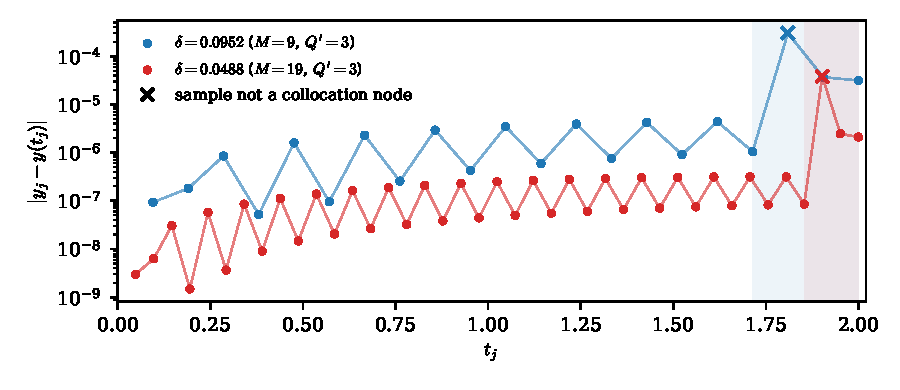
\includegraphics[width=0.78\linewidth]{error_by_sample.pdf}
\caption{Error by sample for $y(t) = g(t) + \int_0^t e^{-(t-s)}y(s)\,ds$ with exact solution
$y=\cos t$, default settings (product, $(2,\{0,1,2\})$, $Q=2$), $T=2$ and $N$ even, so $\Qp = 3$
and $c' = (0,\tfrac23,1)$. Shaded: the final interval. Crosses: the tail sample at offset 1,
which is not a collocation node; it is the largest error and converges one order lower
(between the two resolutions its error falls by about $2^3$, the others by close to $2^4$).
Generated by \code{error\_figure.py}.}
\end{figure}

\end{document}
